\documentclass{article}
\usepackage{palatino}
\usepackage[utf8]{inputenc}
\usepackage[a4paper,top=2cm,bottom=2.5cm,left=1.5cm,right=1.5cm,marginparwidth=1.75cm]{geometry}
%% Language and font encodings
\usepackage[english]{babel}
\usepackage{listings}
\usepackage{float}
\usepackage{pdfpages}
\usepackage{algorithm}
\usepackage[noend]{algpseudocode}

\usepackage{float}
%% Useful packages
\usepackage{relsize}
\usepackage[colorinlistoftodos]{todonotes}
\usepackage[colorlinks=true, allcolors=blue]{hyperref}
\usepackage{listings}
\usepackage{url}
\usepackage{graphicx}
\graphicspath{ {./images/} }
\usepackage{caption}
\usepackage{subcaption}

% MATHEMATICS
\usepackage{enumitem}
\setlist[1]{itemsep=0pt}
\usepackage{array}
\usepackage{amssymb}
\usepackage{amsmath}
\usepackage{arydshln}
\usepackage{amsthm}
\usepackage{mathtools}
\usepackage{accents}
\usepackage{braket}
\usepackage{dsfont}
\usepackage{siunitx}
\usepackage{mathrsfs}
\sisetup{output-exponent-marker=\ensuremath{\mathrm{E}}}

% DEFINITIONS - Mathematics
\def\*#1{\mathbf{#1}}
\def\q{\quad}
\def\t#1{\text{#1}}

\def\bxi{\boldsymbol{\xi}}

\DeclareMathOperator{\sign}{sign}

\title{Rosenblat Perceptron}
\author{Yulan van Oppen (s2640325)\\
Jarvin Mutatiina (s3555631) \\ 
}

\date{\today}

\begin{document}

\maketitle

\section{Introduction}
{\color{blue}
Many applications of machine learning involve binary classification systems, e.g. the spam filter in your email. The basic processing element in such a system is the linear threshold classifier called the perceptron. We very briefly introduce some elementary concepts 

A \textit{dichotomy} is a partition of a set into two disjoint subsets. We denote a dichotomy by $\mathfrak{D}_N^P := \{\bxi^\mu, S^\mu\}_{\mu = 1}^P$, where $\bxi_\mu$ is an $N$-dimensional point and $S^\mu \in \{\pm 1\}$ is the corresponding class label, for $\mu = 1, \ldots, P$. The class label as a function of the data points $\bxi^\mu$ defines a function $S(\bxi)$. Suppose this function is \textit{homogeneously linearly separable}, that is, there exists an $N$-dimensional vector $\*w$ such that
\begin{equation}
	\label{EQ:HLS} \sign(\*w \cdot \bxi^\mu) = S^\mu \q \t{for} \q \mu = 1, \ldots, P.
\end{equation}

The \textit{perceptron (storage) problem} is to find, for such a dichotomy, a vector such that \eqref{EQ:HLS} holds.\\

[ADDITIONAL STUFF]\\}

{\color{orange} \textsc{I think the piece in red should be a little more rigorous, the proposed correction is in blue, above (after an very short introduction). Also, what are linearly separable classes? The above correction would require some small changes in notation} \\}

{\color{red}
Consider a \textit{dichotomy} with a set of observations that are homogeneously linearly separable; then we can deduce that all the  observations fall within the following categories defined by weight vector(w) and the value of the observation, $\xi$.\\
\[
f(x) = 
\begin{cases}
    -1 &  w \cdot \xi > 0 \\
    0,   & w \cdot \xi = 0\\
    1           & w \cdot \xi < 0 
    
\end{cases}
\]}
With this definition/hypothesis, we can assume that any new observations can comfortably fall within the existing partitions. Also Rosenblatt states that if the observation are indeed sampled from two {\color{red}linearly separable classes (??)} then, a separating decision hyper-plane is formed between these two classes. The hyperplane is defined as;
\[
\sum_{i=1}^{n}w_i\cdot x_i + b =0
\]
where \textit{n} is the total number of observations and \textit{b} is the bias. The bias is mainly meant to move the decision boundary away from the origin to cater for correct classification.\\
\noindent Given the distinction between the two classes in the sample space, the Perceptron's problem is to find optimal weights for the input vector that fully classify the inputs into one of the two available classes. In cases of misclassification, the weight vector is adapted until a correct classification is found; as will be described in the next section.\\

Describe the problem

- Goal of the perceptron is to correctly classify a set of input into one of two classes\\
- \textbf{Very brief illustration of a real-life application}\\
- Learning rules- criteria for modifying the weights in scenarios of misclassification \\
\newpage


\section{Notation}

Maybe put this in the intro?

\section{Methodology}
\textbf{This is rough; needs refinement. Feel free to change everything}\\

\begin{algorithm}[h]
\caption{Rosenblatt Perceptron algorithm}\label{alg:perceptron}
Variables: \\
$\mathbf{D} = \{ \xi^\mu, S^\mu \}^p_{\mu=1} $ \Comment{$\xi^\mu$ represents the input vector and $S^\mu$ is the corresponding class label}\\
$w(t) =[w_1(t),w_2(t),w_3(t), \cdots]$ \Comment{weight vector}\\

1. Initialisation w(0) =0;\\
For time steps t=1,2,3,$ \cdots$\\


$ E^\mu = w \cdot \xi^\mu S^\mu  $ \Comment{At every time step compute $E^\mu$}\\

\textbf{If} $E^\mu > 0$ \\
\hspace{10mm}   w(t+1) = w(t) \\
\textbf{else if} $ E^\mu \leq 0 $\\
 w(t+1) = w(t) + $ \frac{1}{N}\xi^{\mu(t)} S^{\mu(t)} $\\

Repeat for all timesteps until optimal weights are found.



\end{algorithm}

- Describe the equations and break down the sections  eg the hebian learning \\
- \textbf{Brief mention of convergence?}\\
- Pseudo code



\section{Results}
\def\Qls{Q_{l.s.}}

In the following section, the number of points $P$ in any given dichotomy will be related to the dimension $N$ of the space under consideration through $P = \alpha N$. We employ the algorithm discussed in the previous section to obtain the fraction of successful runs $\Qls$, as a function of $\alpha$.

Unless specified otherwise, for each figure referred to below, we generate $n_D = 50$ dichotomies $\mathfrak{D}_N^P := \{\bxi^\mu, S^\mu\}_{\mu = 1}^P$. For each dichotomy we allow for a maximum of $n_max = 100$ epochs when using the Rosenblatt algorithm. Moreover, the $N$-dimensional space we consider has default value $N = 20$. When checking whether the local potentials satisfy $E^\mu > c$, $c$ is by default 0. It should be noted that in the "fraction of linearly separable dichotomies" $y$-axis label in each figure, linearly separable is meant as far as can be determined from running the Rosenblatt algorithm with the given settings. The actual fraction is always at least as large as the plotted values.

Holding everything else fixed, varying $n_D$ yields the results depicted in Figure \ref{FIG:VARYND}. Little variation can be observed. Varying $n_{max}$, however, significantly changes the results. This is shown in Figure \ref{FIG:VARYNMAX}. As we vary $N$, the graph of $\Qls$ as a function of $\alpha$ approaches a step function. The point of discontinuity of the approached graph, however, does not appear to lie on the theoretical value $\alpha = 2$. A reason for this is discussed in the next section.

Enforcing a nonzero minimal stability on the solution, i.e. setting $c > 0$, intuitively decreases $\Qls$ for any value of $\alpha$. Figure \ref{FIG:VARYC} supports this intuition. Only for these computations, $n_D$ (which was held fixed) was set to 100. This was in an effort to get rid of large oscillations in the graphs of $\Qls$ as a function of $\alpha$, although some are still present.
\begin{figure}
\centering
\begin{minipage}{.45\textwidth}
  \centering
  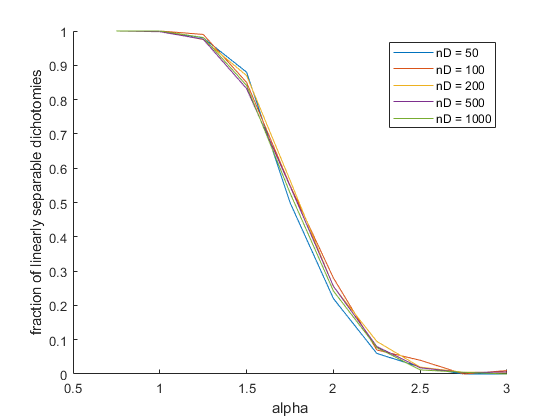
\includegraphics[width=\linewidth]{prob_ls_nD=50_1000}
  \captionof{figure}{Plots of the fraction of linearly separable dichotomies for several values of $n_D$. Here $N = 20$, $n_{max} = 100$, $c = 0$, and $\alpha = 0.75, 1, 1.25, \ldots, 3$.}
  \label{FIG:VARYND}
\end{minipage}\hspace*{.1\textwidth}%
\begin{minipage}{.45\textwidth}
  \centering
  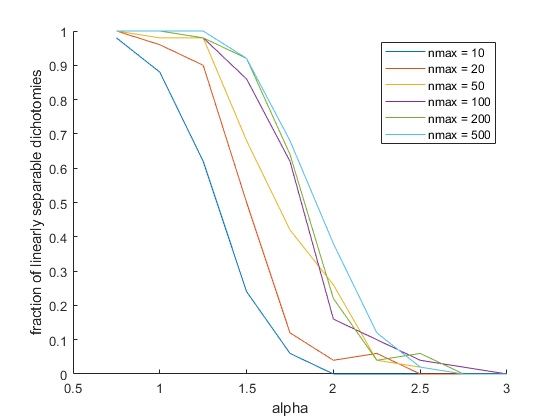
\includegraphics[width=\linewidth]{prob_ls_nmax=10_500}
  \captionof{figure}{Plots of the fraction of linearly separable dichotomies for several values of $n_{max}$. Here $N = 20$, $n_D = 50$, $c = 0$ and $\alpha = 0.75, 1, 1.25, \ldots, 3$.}
  \label{FIG:VARYNMAX}
\end{minipage}
\end{figure}

\begin{figure}
\centering
\begin{minipage}{.45\textwidth}
  \centering
  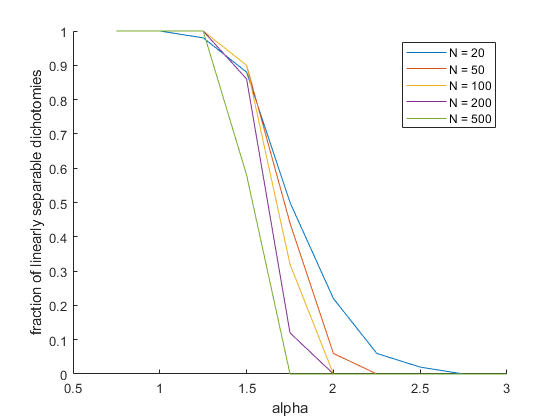
\includegraphics[width=\linewidth]{prob_ls_N=20_500}
  \captionof{figure}{Plots of the fraction of linearly separable dichotomies for several values of $N$. Here $n_{max} = 100$, $n_D = 50$, $c = 0$, and $\alpha = 0.75, 1, 1.25, \ldots, 3$.}
  \label{FIG:VARYN}
\end{minipage}\hspace*{.1\textwidth}%
\begin{minipage}{.45\textwidth}
  \centering
  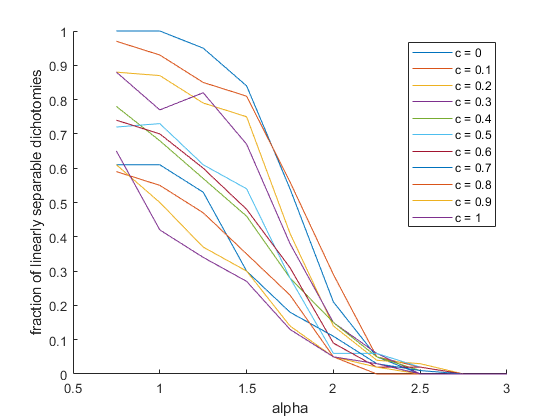
\includegraphics[width=\linewidth]{prob_ls_c=0_1(nD=100)}
  \captionof{figure}{Plots of the fraction of linearly separable dichotomies for several values of $c$. Here $N = 20$, $n_{max} = 100$ and $n_D = 100$, $c = 0$ and $\alpha = 0.75, 1, 1.25, \ldots, 3$.}
  \label{FIG:VARYC}
\end{minipage}
\end{figure}

\textit{Modify the algorithm in order to find also inhomogeneous perceptron solutions by adding a clamped input to all feature vectors. Does Ql.s. change significantly?}


\section{Discussion}
A higher value of $n_D$ yields results that more accurately depict the true mean of the fraction of successful runs of the Rosenblatt algorithm. Figure \ref{FIG:VARYND} showed varying $n_D$ had little effect on the graph of $\Qls(\alpha)$. This suggests that (for most purposes) $n_D = 50$ considers enough different dichotomies for trustworthy results.

We know from theory that the Rosenblatt algorithm converges for linearly separable dichotomies in finitely many iterations, and for $\alpha <2$ this is the case with probability 1. Finitely many, however, can turn out to be quite a lot. Increasing $n_{max}$ increases the probability of convergence within $n_{max}$ iterations. For $n_{max} = 100$ (our default value), we see the graph of $\Qls(\alpha)$ in Figure \ref{FIG:VARYNMAX} has generally lower values than its theoretical counterpart. This difference vanishes as $n_{max}$ is sufficiently increased.

This observation moreover explains why the step function approached by the graphs in Figure \ref{FIG:VARYN} does not seem to have a discontinuity at $\alpha = 2$, but rather at $\alpha \approx 1.5$. Taking $n_max$ considerably larger, i.e $n_max = 1000$, shows a low $n_{max}$ really is the cause of this phenomenon. See Figure \ref{FIG:LARGEN}.

In the previous section, we remarked that it was intuitive that $\Qls$ decreased when increasing $c$. This is because for $0 < c_1 < c_2$, a solution with minimal stability $c_2$ is also a solution with minimal stability $c_1$. Hence, the probability that the algorithm has a successful run cannot increase when $c$ is increased.

[HERE GOES THE PART FOR THE LAST BONUS QUESTION] 


\nocite{*}
\bibliographystyle{plain}
\bibliography{bibfil}
\end{document}
